\documentclass[border=3pt,tikz]{standalone}
\usepackage{amsmath}
\begin{document}
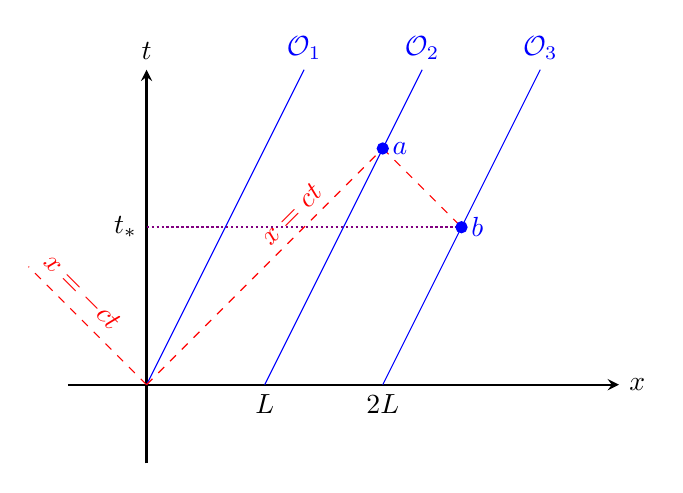
\begin{tikzpicture}[]
    \draw[thick,->,>=stealth] (0, -1) -- (0, 4) node[above] {$t$};
    \draw[thick,->,>=stealth] (-1, 0) -- (6, 0) node[right] {$x$};
    \draw[blue] (0,0)-- (2, 4) node[above] {$\mathcal{O}_1$};
    \draw[blue] (1.5, 0) -- (3.5, 4) node[above] {$\mathcal{O}_2$};
    \draw[blue] (3, 0)-- (5, 4) node[above] {$\mathcal{O}_3$};
    \draw[red, dashed] (0,0)-- (2, 2) node[above, rotate=45] {$x=ct$} -- (3, 3);
    \draw[red, dashed] (0,0)-- (-1, 1) node[above, rotate=-45] {$x=-ct$} -- (-1.5, 1.5);
    \draw[red, dashed] (3,3) -- (4, 2);
    \draw[thick, violet, densely dotted] (0, 2) -- (4, 2) ;
    \filldraw[blue] (3, 3) circle(2px) node[right] {$a$};
    \filldraw[blue] (4, 2) circle(2px) node[right] {$b$};
    \node[below] at (1.5, 0) {$L$};
    \node[below] at (3 , 0) {$2L$};
    \node[left] at (0, 2) {$t_\ast$};
    \end{tikzpicture}
\end{document}